% !TeX root = ../../Thesis.tex
\chapter{Theory}
\label{chp:theory}

This chapter aims to equip the reader with the tools they need to read, and to engage critically with, the rest of the thesis. By the end of this chapter, the reader should be familiar with the following concepts and methods:
\begin{enumerate}
	\item Stimulated Raman scattering (\acrshort{SRS}) as a three-wave parametric instability.
	\item The difference between convective and absolute SRS, and how we can quantify their gain.
	\item The difference between fluid and kinetic SRS, and how we can use $\kld$ to delineate these two regimes.
	\item The effect of large trapped-particle populations on SRS, including the growth of additional resonant modes.
\end{enumerate}


\section{Pre-requisites}
This section provides a minimal set of pre-requisites I will be assuming in this chapter. First up, we have Maxwell's equations in differential form:



\begin{equation}
\nabla \times \vec{E}=-\frac{\partial \vec{B}}{\partial t} \text{\,\,\,\,\,\,\,\,\,(Faraday-Lenz Law)}
\end{equation}

\begin{equation}
\nabla \times \vec{B}=\mu_{0} \vec{j}+\frac{1}{c^{2}} \frac{\partial \vec{E}}{\partial t}
\text{\,\,\,\,\,\,\,\,\,(Ampere-Maxwell Law)}
\end{equation}

\begin{equation}
\nabla \cdot \vec{B}=0 \text{\,\,\,\,\,\,\,\,\,(No Magnetic Monopoles)}
\end{equation}

\begin{equation}
\nabla \cdot \vec{E}=\frac{\rho}{\epsilon_{0}} \text{\,\,\,\,\,\,\,\,\,(Gauss's Law)}.
\end{equation} These describe the evolution of the vector fields $[\vec{E}(\vec{x},t),\vec{B}(\vec{x},t))]$ using the mathematical notation $\nabla = \left(\frac{\partial}{\partial x},\frac{\partial}{\partial y},\frac{\partial}{\partial z} \right)$ to denote the scalar function divergence $(\nabla \cdot)$ and the vector function curl $(\nabla \times)$. The charge density $\rho$ and current density $\vec{j}$ are most properly calculated by summing the contributions of the exact phase-space coordinates of every particle in the plasma. However, we can make an approximation and assume that that the phase space is continuous and take an average to get the distribution function $f(\vec{x},\vec{v},t)$. We can now define $\rho$ and $\vec{j}$ in terms of the distribution function like so:

\begin{equation}
\rho= q \int d \vec{v} f(\vec{x},\vec{v},t)
\end{equation}

\begin{equation}
\vec{j} = q \int d \vec{v} \vec{v} f(\vec{x},\vec{v},t).
\end{equation}

In order to close the Maxwell equations, we need an equation which tells us how the distribution function evolves in terms of $[\vec{E}(\vec{x},t),\vec{B}(\vec{x},t))]$. An entire two weeks of kinetic theory lectures later, we end up with the Vlasov equation for a collisionless plasma:

\begin{equation}
 	\frac{\partial f}{\partial t}+\vec{v} \cdot {\nabla} f+\frac{q}{m}\left(\vec{E}+\frac{\vec{v} \times \vec{B}}{c}\right) \cdot \frac{\partial f}{\partial \vec{v}}=0
\end{equation} By taking moments of the Vlasov equation (and moving to 1D for brevity), we obtain the following reduced description of the plasma in terms of a fluid of electrons: 
\begin{equation}
\frac{\partial n}{\partial t}+\frac{\partial}{\partial x}(n u)=0 \text{\,\,\,\,\,\,\,\,\,(0th moment: Continuity equation)}
\end{equation}

\begin{equation}
m_e n \left(\frac{\partial u}{\partial t} + u\frac{\partial}{\partial x}u\right)=-\frac{\partial P}{\partial x}+q E_{x} n \text{\,\,\,\,\,\,\,\,\,(1st moment: Momentum equation)}.
\end{equation} Where $n$ is the number density (calculated by taking the zeroth moment of the distribution function); $u$ is the macroscopic flow velocity (calculated by taking the first moment of the distribution function); and $P$ is a scalar pressure. In order to close this st of equations, we require an expression for the scalar pressure $P$ that does not introduce any higher moments of the distribution function. Typically in this thesis the timescales are such that thermal conduction can be neglected, and we assume that the process is adiabatic. This means that our final equation takes the form:

\begin{equation}
\frac{d}{dt}\left(\frac{P}{n^{\gamma}}\right) = 0,
\end{equation} with $\gamma = C_p/C_v = 1 + 2/s = 3$ in one dimension. 

We must also recall the fundamental time and length scales associated with a plasma: the plasma frequency and the Debye length. The plasma frequency describes the natural frequency of oscillation of (generally) electrons in a cold plasma, its expression in terms of the electron number density can be derived by considering the displacement of a block of plasma and considering the restoring forces, to give:

\begin{equation}
	\omega_{pe} = \sqrt{\frac{n_e e^2}{m_e \epsilon_0}}.
\end{equation} This fundamental time-scale allows us to define a fundamental length-scale based on how far a particle with thermal velocity $v_{\text{th}}$ can travel in one oscillation period.

\begin{equation}
	\lambda_D = \frac{v_{\mathrm{th}}}{\omega_{pe}} \propto \left(\frac{\mathrm{temperature}}{\mathrm{density}}\right)^{1/2}.
\end{equation}\label{eqn:debye} The thermal velocity is given by:
\begin{equation}
	v_{\text{th}} = \sqrt{\frac{\gamma k_BT_e}{m_e}}
\end{equation}\label{eqn:vth}, where $k_B$ is the Boltzmann constant

Linear approximation means reglecting, in your equations, quadratic or higher order terms in the peturbation variables. Also assume that the peturbation is harmonic both in space and time.
\section{Fluid theory of three-wave instabilities}
Equipped with this brief revision of the fundamental relationships which describe a plasma, we can now move onto the theory behind our object of study: stimulated Raman scattering.

\subsection{Dispersion curves and linear modes}

One obvious thing to do, now that we have the fluid equations for an electron plasma, would be to look for normal modes of the system. These describe oscillations in which all variables vary sinusoidally with the same frequency, meaning that they can be written as $n(x,t) = n_1(x)\text{exp}(-i\omega t)$
A non-magnetised, two-species (electron-ion) plasma supports two electrostatic (no time-varying magnetic fields) modes and one electromagnetic mode. 

\begin{equation}\label{eqn:bohm-gross}
	\omega^{2}=\omega_{p e}^{2}+3 k^{2} v_{\text{th}}^{2} \text{\,\,\,\,\,\,\,\,\,(Electron plasma wave)}
\end{equation}

\begin{equation}
 \omega =  c_{si} k \text{\,\,\,\,\,\,\,\,\,(Ion acoustic wave)}
\end{equation}

\begin{equation}
 \omega^{2}=\omega_{p e}^{2}+c^2k^{2} \text{\,\,\,\,\,\,\,\,\,(Electromagnetic wave)}
\end{equation}

With these three waves, we find the following three-wave parametric instabilities:

\begin{alignat*}{2}
	 	&\text{EMW1} \rightarrow \text{EPW} + \text{EMW2} &\text{\,\,\,\,\,\,\,\,\,(Stimulated Raman Scattering)}\\
	 	&\text{EMW1} \rightarrow \text{IAW} + \text{EMW2} &\text{\,\,\,\,\,\,\,\,\,(Stimulated Brillouin Scattering)}\\
	 	&\text{EMW1} \rightarrow \text{EPW1} + \text{EPW2} &\text{\,\,\,\,\,\,\,\,\,(Two-Plasmon Decay)}\\
	 	&\text{EPW1} \rightarrow \text{EPW2} + \text{IAW} &\text{\,\,\,\,\,\,\,\,\,(Langmuir Decay Instability)}\\
	 	&\text{EMW} \rightarrow \text{EPW} + \text{IAW} &\text{\,\,\,\,\,\,\,\,\,(The Parametric Instability)}\\
\end{alignat*}



\subsection{Stimulated Raman scattering}


\subsubsection{Rosenbluth gain}

Since the instability we are concerned with is convective, we would like to understand what the maximum wave amplitude is for the daughter waves, according to the linear theory, in order to determine how SRS will grow in the fluid regime.

The derivation below follows the the steps laid out in \citet{Nishikawa1976}, with the following adapatations for this thesis:some steps written out in more explicit detail; notation changes, to improve the readability; and minor typographical corrections. 

We use our physical understanding of the system make the following assumptions:
\begin{enumerate}
	\item undamped EMW $\Gamma_1 = 0$
	\item strong damping and slow convection of EPW
	\item constant source at 0, maximum value at $+\infty$
	\item perfect matching at $x=0$, assume kappa is well-approximated by 
	$\kappa(x) = \kappa'(0)x$.
\end{enumerate}

Consider a three-wave parametric instability that takes place in a plasma slab with a density gradient in $x$ with a uniform pump. The density gradient leads to $x$-varying wavenumbers for the waves, so we define the `wavenumber mismatch' as $\kappa = k_0(x) - k_1(x) - k_2(x)$, where perfect matching is defined by the condition $\kappa(x=0) = 0$ and we insist that $\kappa = \kappa' x$. The daughter waves can be described by the following pair of partial differential equations:

\begin{equation}
 \left(\frac{\partial}{\partial t} + v_1\frac{\partial}{\partial x} + \Gamma_1 \right)a_1 = \gamma_0a_2\text{exp}\left(\frac{i\kappa'x^2}{2}\right)
\end{equation}

\begin{equation}
 \left(\frac{\partial}{\partial t} + v_2\frac{\partial}{\partial x} + \Gamma_2 \right)a_2 = \gamma_0a_1\text{exp}\left(\frac{-i\kappa'x^2}{2}\right);
\end{equation} 
where $\Gamma_{1,2}$ are the damping rates; $a_{1,2}$ the action amplitudes; and $v_{1,2}$ the group velocities of the two waves. 

WHAT ARE WE TRYING TO DO, WHAT MOTIVATES THIS TRANSFORM?

Recalling the definition of the Laplace transform of a function $f(t)$: $L\{f(t)\}= F(p) = \int_0^\infty e^{-pt} f(t) dt$ we take the Laplace transform of these equations to get






\subsection{Stimulated Brillouin scattering}
Since SBS is only important in Chapter \ref{chp:magSRS}, we will only give a very brief overview of it here.


\section{Kinetic theory of three-wave instabilities}


\subsection{Landau damping}


Unfortunately, by looking for normal modes, we have forced ourselves to find normal modes and we have ignored the possibility of damped oscillations in the system. Considering the electron plasma wave as an initial value problem 
A key aspect of quasilinear theory is its identification of the distinction between reso-
nant and non-resonant particles, scattering and diffusion \citep{Sagdeev2018}.

\subsection{Nonlinear frequency shift}
non-linear basis for trapping induced SRS modes found in \cite{Rose2001}



\section{Three-wave instabilities in a magnetic field}

In a magnetic field, we can define a new fundamental frequency. The cyclotron frequency is given by:
\begin{equation}
\omega_c = \frac{eB_0}{m_ec}.
\end{equation}

The dispersion relation for the upper-hybrid 

\section{Autoresonance}

\begin{figure}[ht]
    \centering
    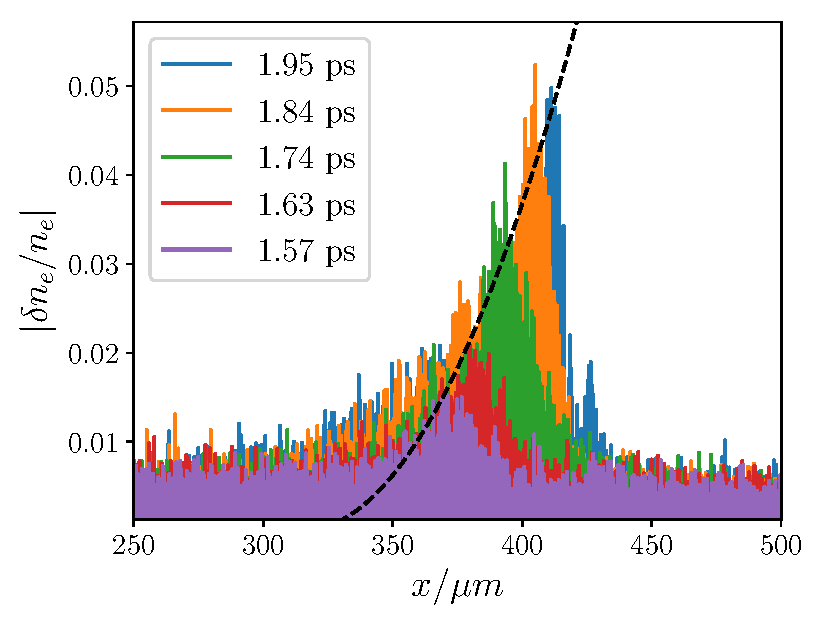
\includegraphics[width=0.8\columnwidth]{Chapters/C2_Theory/AR_diagnostic.pdf}
    \caption{Example of autoresonant growth in an EPOCH simulation with parameters: $n_{min} = 0.06 n_{\text{crit}}$; $n_{max} = 0.17 n_{\text{crit}}$; $T_e = 4.5\si{keV}$; $\text{nPPC}=10,000$; $I_0 = 2 \times 10^{15}\si{\watt / \centi\metre^2}$. Black dashed line comes from Chapman \textit{et al.} \citep{Chapman2012} formula.}
    \label{fig:AR_diagnostic}
\end{figure}{}

%\bibliographystyle{plainnat}
%\bibliography{Chapters/C2_Theory/Theory}
